\section{Desarrollo}
\subsection{C\'odigo 1: Control ON/OFF con Transistor BJT}
Este c\'odigo implementa un control b\'asico de encendido y apagado de la bombilla utilizando un transistor BJT BD235 como interruptor, como se muestra en la Figura \ref{fig:codigo-bjt}.
\begin{figure}[H]
	\centering
	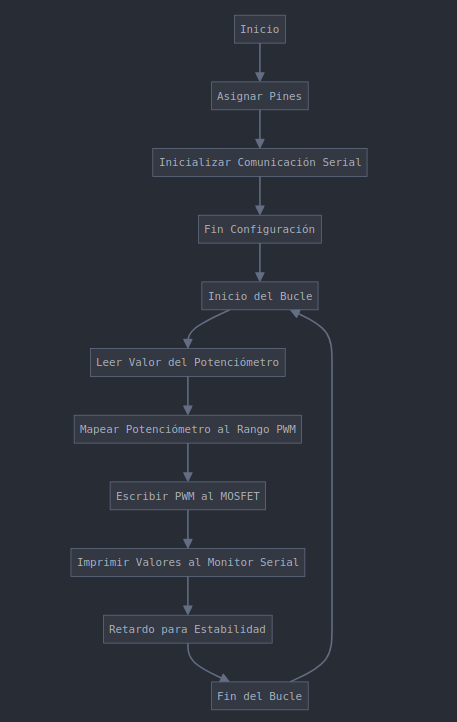
\includegraphics[width=0.3\textwidth]{images/dbjt}
	\caption{Diagrama de Flujo BJT}
	\label{fig:flujobjt}
\end{figure}

\begin{figure}[H]
	\centering
	\begin{lstlisting}[
		language=C++,
		basicstyle=\ttfamily\scriptsize,
		numbers=left,
		numberstyle=\tiny\color{gray},
		backgroundcolor=\color{codeBackground},
		commentstyle=\color{comentarios},
		keywordstyle=\color{identificador},
		stringstyle=\color{cadena},
		emph={pinMode,digitalWrite,HIGH,LOW},
		emphstyle={\color{blue}\bfseries},
		frame=single,
		frameround=tttt,
		rulecolor=\color{arduinoBlue},
		xleftmargin=3mm,
		xrightmargin=2mm,
		breaklines=false,
		columns=fullflexible,
		keepspaces=true,
		basewidth=0.5em]
//---------------------------
// Definicion del pin para 
// el transistor BD235 como
// interruptor digital
//---------------------------
const int PIN_BJT = 1;    

//---------------------------
// Configuracion inicial
//---------------------------
void setup() {
	pinMode(PIN_BJT, OUTPUT);
	digitalWrite(PIN_BJT, LOW);
}

//---------------------------
// Bucle principal
//---------------------------
void loop() {
	digitalWrite(PIN_BJT, HIGH);
	delay(1000);  
	
	digitalWrite(PIN_BJT, LOW);
	delay(1000);  
}
	\end{lstlisting}
	\caption{C\'odigo de control ON/OFF con transistor BD235}
	\label{fig:codigo-bjt}
\end{figure}

\subsection{Análisis del Código 1}
El código mostrado en la Figura \ref{fig:codigo-bjt} implementa un sistema de control digital básico usando un transistor BJT. Los elementos principales son:

\begin{itemize}
	\item \texttt{PIN\_BJT}: Pin digital 1 que controla la base del transistor
	\item \texttt{digitalWrite()}: Función que controla el estado del pin (HIGH/LOW)
	\item \texttt{delay()}: Función que genera pausas de 1 segundo entre estados
	\item \texttt{setup()}: Configura el pin como salida e inicia en estado LOW
	\item \texttt{loop()}: Alterna el estado del transistor cada segundo
\end{itemize}

\subsection{Elementos del Circuito con BJT}
Para implementar el control mostrado en la Figura \ref{fig:codigo-bjt}, se requiere:
\begin{figure}[H]
	\centering
	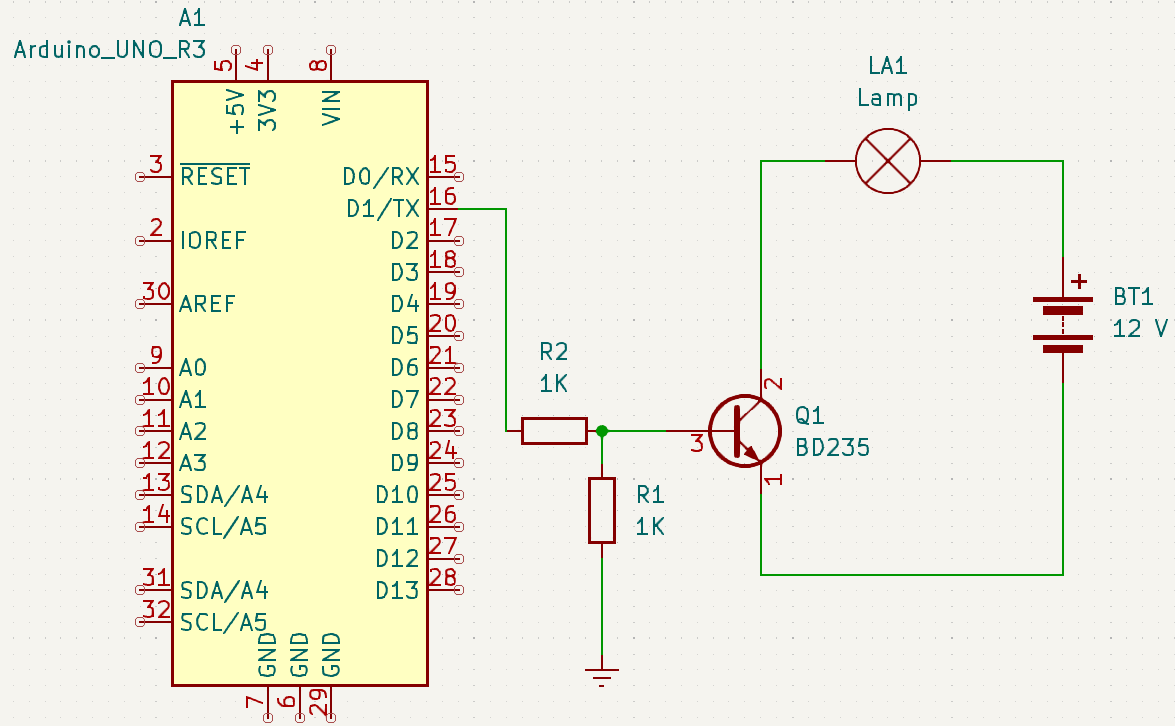
\includegraphics[width=0.3\textwidth]{images/esquematico1}
	\caption{Diagrama de Conexiones BJT BD235}
	\label{fig:diagramaBJT}
\end{figure}
\begin{itemize}
	\item Transistor BD235 (BJT)
	\item Resistencia de \SI{100}{\ohm} para la base
	\item Bombilla de \SI{12}{\volt}/\SI{10}{\watt}
	\item Fuente de alimentación de \SI{12}{\volt}
\end{itemize}

\begin{figure}[H]
	\centering
	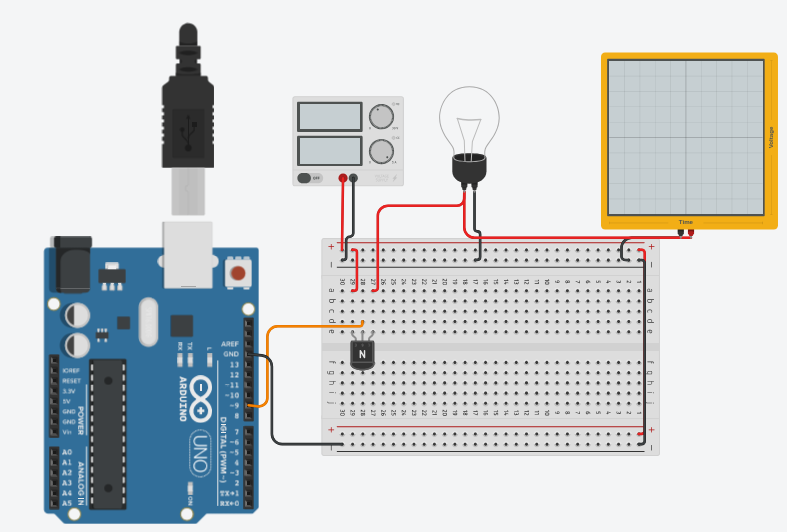
\includegraphics[width=0.3\textwidth]{images/conexion1}
	\caption{Diagrama de Conexiones Físicas BJT}
	\label{fig:conexionbjt}
\end{figure}

\subsection{Funcionamiento del Control ON/OFF}
El código implementa un control básico ON/OFF que:
\begin{enumerate}
	\item Enciende la bombilla (HIGH) durante 1 segundo
	\item Apaga la bombilla (LOW) durante 1 segundo
	\item Repite el ciclo indefinidamente
\end{enumerate}

\subsection{Diagrama de Tiempo BJT}
\begin{verbatim}
	Voltaje      _____       _____      
	Base     ___|     |_____|     |_____
	
	ON  OFF  ON  OFF  ON  OFF  ON  OFF
	Tiempo   0s  1s   2s  3s   4s  5s  
\end{verbatim}

\subsection{Ventajas y Características del BJT}
\begin{itemize}
	\item Control digital simple y robusto
	\item Ideal para aplicaciones de encendido/apagado
	\item Bajo consumo en modo de corte
	\item Protección inherente por la resistencia de base
\end{itemize}

\subsection{Limitaciones del Control BJT}
\begin{itemize}
	\item Solo permite control ON/OFF (no dimming)
	\item Puede requerir disipador según la carga
	\item Mayor pérdida de potencia que MOSFET
	\item Requiere corriente de base continua
\end{itemize}

\subsection{Aplicaciones Típicas del Control ON/OFF}
Este tipo de control es ideal para:
\begin{itemize}
	\item Iluminación básica ON/OFF
	\item Control de cargas resistivas
	\item Sistemas de señalización
	\item Automatización simple
\end{itemize}

\subsection{Código 2: MOSFET}
\begin{figure}[H]
	\centering
	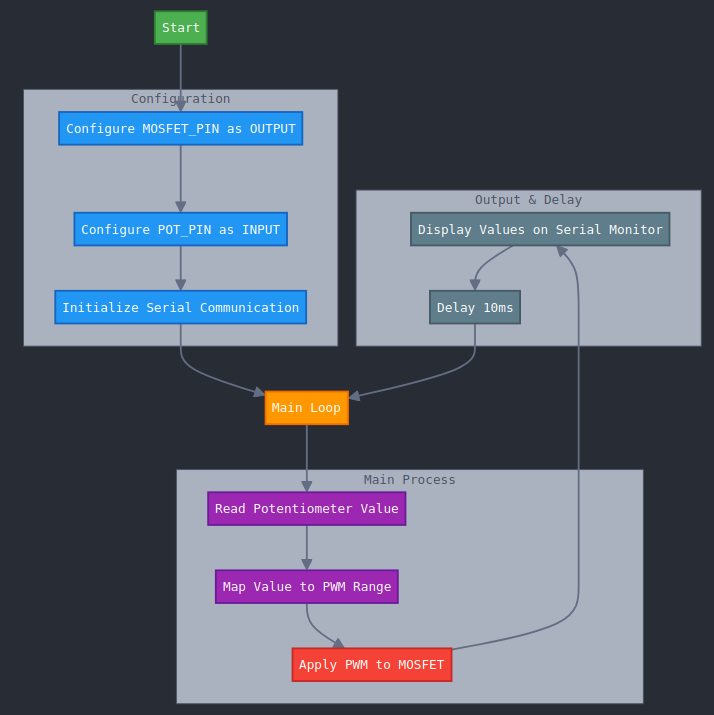
\includegraphics[width=0.3\textwidth]{images/flujom}
	\caption{Diagrama de Flujo MOSFET}
	\label{fig:flujomosfet}
\end{figure}

\begin{figure}[H]
	\centering
	\begin{lstlisting}[
		language=C++,
		basicstyle=\ttfamily\scriptsize,
		numbers=left,
		numberstyle=\tiny\color{gray},
		backgroundcolor=\color{codeBackground},
		commentstyle=\color{comentarios},
		keywordstyle=\color{identificador},
		stringstyle=\color{cadena},
		emph={pinMode,digitalWrite,analogWrite,analogRead,map,Serial,begin,print,println,HIGH,LOW},
		emphstyle={\color{blue}\bfseries},
		frame=single,
		frameround=tttt,
		rulecolor=\color{arduinoBlue},
		xleftmargin=3mm,
		xrightmargin=2mm,
		breaklines=false,
		columns=fullflexible,
		keepspaces=true,
		basewidth=0.5em]
//---------------------------
// Definicion de pines para
// control con MOSFET IRLZ14
//---------------------------
const int MOSFET_PIN = 3;    
const int POT_PIN = A0;      

//---------------------------
// Variables para el control
//---------------------------
int valorPotenciometro = 0;  
int valorPWM = 0;           

//---------------------------
// Configuracion inicial
//---------------------------
void setup() {
	pinMode(MOSFET_PIN, OUTPUT);    
	pinMode(POT_PIN, INPUT);        
	Serial.begin(9600);
}

//---------------------------
// Bucle principal
//---------------------------
void loop() {
	valorPotenciometro = analogRead(POT_PIN);
	valorPWM = map(valorPotenciometro, 
	0, 1023, 0, 255);
	analogWrite(MOSFET_PIN, valorPWM);
	
	Serial.print("Potenciometro:");
	Serial.print(valorPotenciometro);
	Serial.print("PWM:");
	Serial.println(valorPWM);
	
	delay(10);
}
	\end{lstlisting}
	\caption{C\'odigo de control variable con MOSFET IRLZ14 y potenci\'ometro}
	\label{fig:codigo-mosfet}
\end{figure}

\subsection{An\'alisis del C\'odigo 2}
El c\'odigo mostrado en la Figura \ref{fig:codigo-mosfet} implementa un sistema de control anal\'ogico usando un MOSFET. Los elementos principales son:

\begin{itemize}
	\item \texttt{MOSFET\_PIN}: Pin PWM 3 que controla el gate del MOSFET
	\item \texttt{POT\_PIN}: Pin anal\'ogico A0 que lee el potenci\'ometro
	\item \texttt{map()}: Funci\'on que convierte el rango del potenci\'ometro (0-1023) al rango PWM (0-255)
	\item \texttt{analogWrite()}: Genera la se\~nal PWM para controlar la intensidad
\end{itemize}

\subsection{Conexiones del Hardware}
\subsubsection{Circuito con BJT (BD235)}
Basado en el c\'odigo de la Figura \ref{fig:codigo-bjt}, las conexiones requeridas son:
\begin{itemize}
	\item Base $\rightarrow$ Pin 1 (con resistencia \SI{100}{\ohm})
	\item Colector $\rightarrow$ Bombilla $\rightarrow$ \SI{12}{\volt}
	\item Emisor $\rightarrow$ GND
\end{itemize}

\subsubsection{Circuito con MOSFET (IRLZ14)}
Para implementar el control mostrado en la Figura \ref{fig:codigo-mosfet}, se requieren las siguientes conexiones:
\begin{figure}[H]
	\centering
	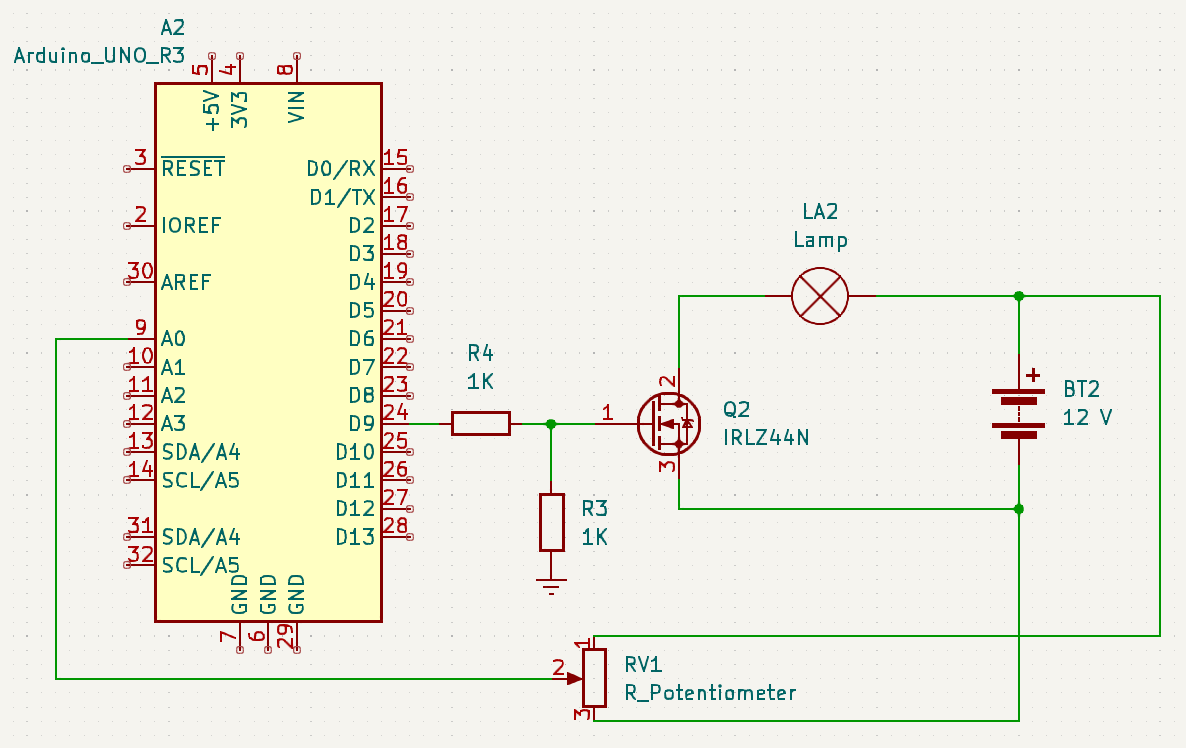
\includegraphics[width=0.3\textwidth]{images/esquematico2}
	\caption{Diagrama de Conexiones MOSFET IRLZ14}
	\label{fig:diagramaMOSFET}
\end{figure}
\begin{itemize}
	\item Gate $\rightarrow$ Pin 3 (con resistencia \SI{100}{\ohm})
	\item Drain $\rightarrow$ Bombilla $\rightarrow$ \SI{12}{\volt}
	\item Source $\rightarrow$ GND
	\item Potenci\'ometro:
	\begin{itemize}
		\item Terminal central $\rightarrow$ A0
		\item Terminal superior $\rightarrow$ \SI{5}{\volt}
		\item Terminal inferior $\rightarrow$ GND
	\end{itemize}
\end{itemize}
\begin{figure}[H]
	\centering
	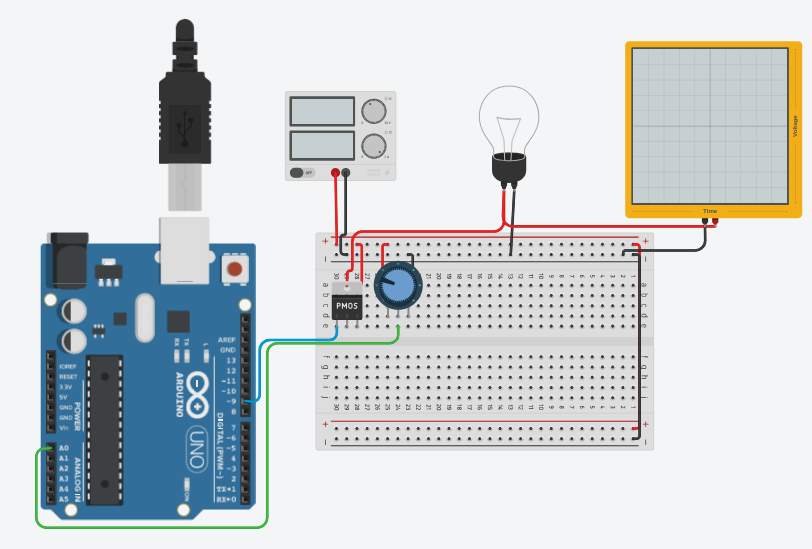
\includegraphics[width=0.3\textwidth]{images/conexion2}
	\caption{Diagrama de Conexiones MOSFET}
	\label{fig:conexionesmosfet}
\end{figure}

\subsection{Consideraciones T\'ecnicas}
Para el correcto funcionamiento de los circuitos mostrados en las Figuras \ref{fig:codigo-bjt} y \ref{fig:codigo-mosfet}, se deben tener en cuenta los siguientes aspectos:
\begin{itemize}
	\item La resistencia en la base/gate es crucial para proteger el transistor/MOSFET
	\item El MOSFET IRLZ14 opera con voltajes de gate bajos, compatible con la se\~nal de \SI{5}{\volt} del Arduino
	\item El transistor BD235 maneja hasta \SI{2}{\ampere}, suficiente para la bombilla de \SI{10}{\watt}
	\item La fuente de \SI{12}{\volt} debe poder suministrar al menos \SI{1}{\ampere}
\end{itemize}

\subsection{Problemas Comunes y Soluciones}

\subsubsection{Circuito BJT}
Para el circuito de la Figura \ref{fig:codigo-bjt}, los problemas comunes incluyen:
\begin{itemize}
	\item \textbf{Problema}: La bombilla no enciende
	\begin{itemize}
		\item Verificar polaridad del transistor
		\item Medir voltaje en la base (\SI{0.7}{\volt} aprox.)
		\item Comprobar resistencia de \SI{100}{\ohm}
	\end{itemize}
	
	\item \textbf{Problema}: Transistor se calienta
	\begin{itemize}
		\item Verificar corriente de base
		\item Comprobar saturaci\'on del transistor
		\item Considerar uso de disipador
	\end{itemize}
\end{itemize}

\subsubsection{Circuito MOSFET}
Para el circuito de la Figura \ref{fig:codigo-mosfet}, los problemas típicos son:
\begin{itemize}
	\item \textbf{Problema}: Control irregular
	\begin{itemize}
		\item Verificar conexi\'on del potenci\'ometro
		\item Comprobar resistencia de gate
		\item Asegurar uso de pin PWM correcto
	\end{itemize}
	
	\item \textbf{Problema}: MOSFET se calienta
	\begin{itemize}
		\item Verificar frecuencia PWM
		\item Comprobar voltaje gate-source
		\item Considerar disipador si es necesario
	\end{itemize}
\end{itemize}

\subsection{Medidas de Seguridad}
Para garantizar la operación segura de los circuitos presentados en las Figuras \ref{fig:codigo-bjt} y \ref{fig:codigo-mosfet}:

\begin{itemize}
	\item \textbf{Antes de energizar}:
	\begin{itemize}
		\item Verificar todas las conexiones
		\item Comprobar polaridad de componentes
		\item Asegurar resistencias limitadoras
	\end{itemize}
	
	\item \textbf{Durante la operaci\'on}:
	\begin{itemize}
		\item No tocar componentes energizados
		\item Mantener ventilaci\'on adecuada
		\item Monitorear temperatura de componentes
	\end{itemize}
\end{itemize}